\documentclass[]{jsarticle}
\usepackage[dvipdfmx]{graphicx}

\title{電子回路設計・製作 課題5-2-4}
\author{32番 平田 蓮}
\date{2020年7月30日}

\begin{document}
\maketitle
\section{作品名}
    リアルタイム電卓

\section{設計仕様案}
    \subsection{回路図と動作}
        図\ref{fig:circuit}に回路図を示す.
        Arduino, 4$\times$4キーパッド, 16$\times$2液晶ディスプレイ(LCD)で構成されている.
        キーパッドでは0から9の数字, $+ - \times \div$の記号, 一文字削除, 全削除を入力することができる.
        数字キー以外のの対応は,
        (A, $+$), (B, $-$), ($*$, $\times$), (D, $\div$), (\#, 一文字削除), (C, 全削除)である.

        キーパッドから入力されると, その結果がLCDの上段に示される.
        同時に, 上段の計算結果が下段に表示される.

        LCDにつないでいるLED用の制限抵抗は, LEDの順方向電圧を1.76 V,
        順方向電流を18 mAとすると,$\displaystyle\frac{5 - 1.76}{18 \times 10^{-3}} = 180 \Omega$と計算できる.

        \begin{figure}[h]
            \centering
            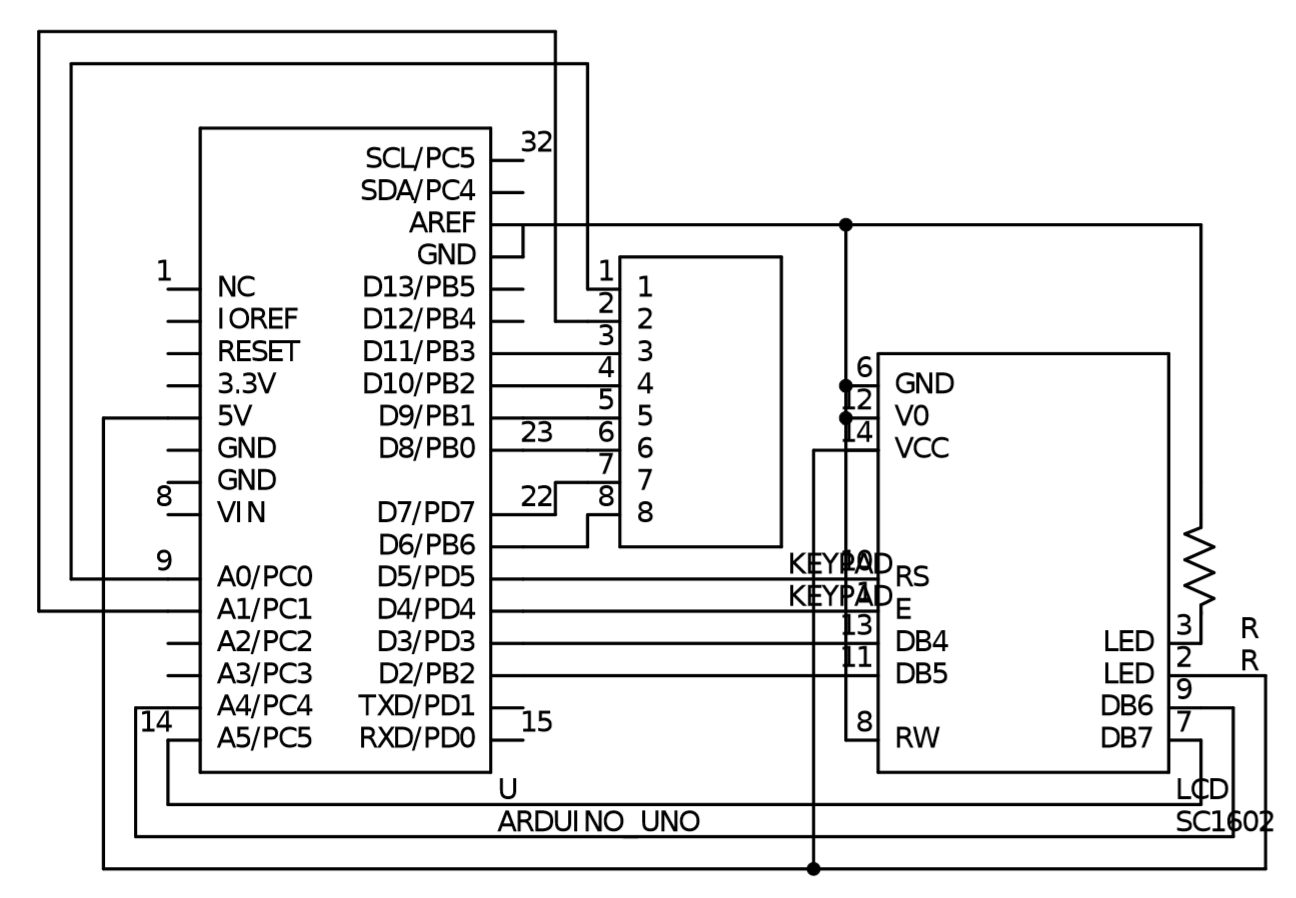
\includegraphics[width=12cm]{images/circuit.png}
            \caption{回路図}
            \label{fig:circuit}
        \end{figure}

    \subsection{フローチャートと動作}
        図\ref{fig:flowchart}にフローチャートを示す.

        入力されるキーに対して, 削除キーであれば入力の削除動作を行い,
        その後値を算出して出力するものである.

        \begin{figure}[h]
            \centering
            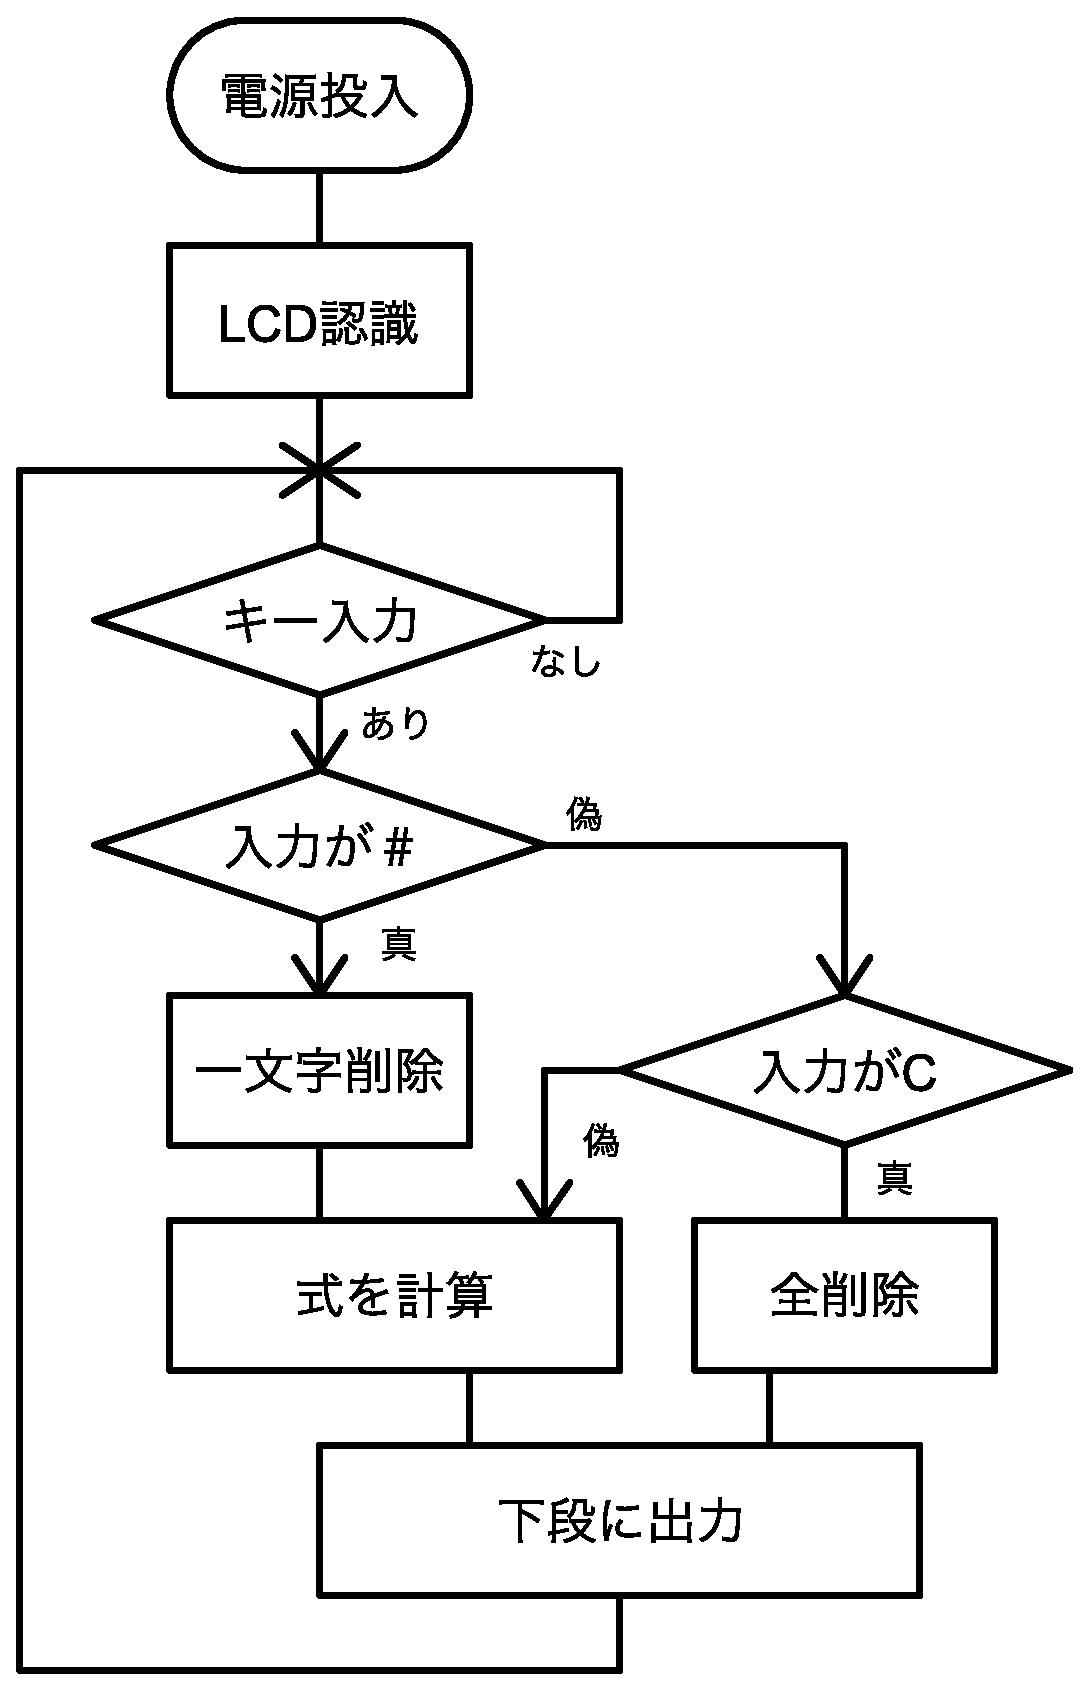
\includegraphics[width=7cm]{images/flowchart.eps}
            \caption{フローチャート}
            \label{fig:flowchart}
        \end{figure}

\section{進捗状況}
    実際の回路はほぼ完成している状況である.
    今後は時間に余裕を持って実験レポートを進めていきたい.

\end{document}